% main_1_relaxation
\begin{figure}[t]
\centering
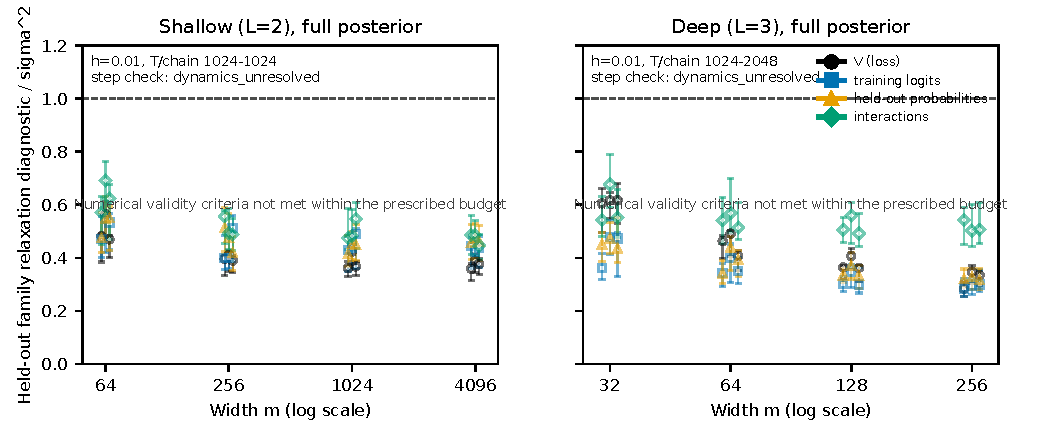
\includegraphics[width=\linewidth]{figures/main_1_relaxation.pdf}
\caption{Width dependence of observable relaxation under unrestricted posterior dynamics. The horizontal axes give network width for the one-hidden-layer and two-hidden-layer models, at fixed n=128. Vertical values are cross-evaluated family autocorrelation integrals in the physical-time convention of the adjusted Gaussian-preserving Langevin proposal, normalized by the prior variance. Families contain the likelihood potential, eight training logits, eight held-out probabilities, and four fixed head--hidden interactions. Thin points and lines show three independent data/center replicates; the thick line is their median, and error bars show within-target Monte Carlo uncertainty. Hollow points did not meet the validity criteria. The horizontal line at one is the continuous Gaussian linear-observable timescale. The production steps were shallow h=0.01, deep h=0.01; endpoint step-halving checks: shallow: dynamics\_unresolved after one refinement, deep: dynamics\_unresolved after one refinement. Over the tested width range, shallow: interactions: unresolved (3 of 3 replicate ratios invalid); V (loss): unresolved (3 of 3 replicate ratios invalid); held-out probabilities: unresolved (3 of 3 replicate ratios invalid); training logits: unresolved (3 of 3 replicate ratios invalid); deep: interactions: unresolved (3 of 3 replicate ratios invalid); V (loss): unresolved (3 of 3 replicate ratios invalid); held-out probabilities: unresolved (3 of 3 replicate ratios invalid); training logits: unresolved (3 of 3 replicate ratios invalid). These finite-observable diagnostics do not estimate the optimal PI coefficient, and no global head or hidden-layer restriction was imposed on the chains.}
\label{fig:main_1_relaxation}
\end{figure}

% main_2_entropy
\begin{figure}[t]
\centering
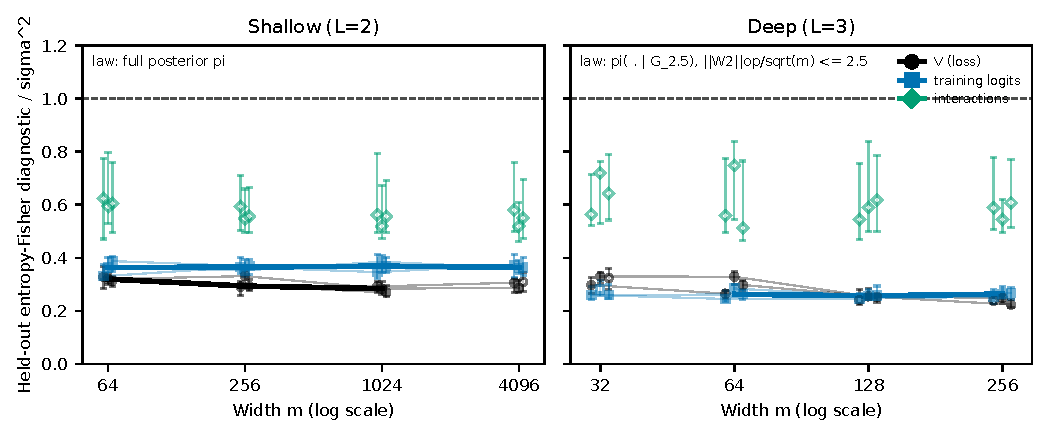
\includegraphics[width=\linewidth]{figures/main_2_entropy.pdf}
\caption{Finite-probe entropy--Fisher diagnostics for the final LSI domains. For each standardized smooth probe f and fixed tilt t in {-1,-0.5,0.5,1}, we form the normalized density r proportional to exp(tf) relative to the shallow posterior or the deep posterior conditioned on the later-hidden-layer spectral event. The vertical axis reports held-out family estimates of 2 Ent(r)/E[r||grad log r||\^{}2], divided by the prior variance; the horizontal axis is width. The head and first hidden layer remain unrestricted in both panels. Probe selection and evaluation use separate chain folds. The value-one line is attained by Gaussian linear tilts and is a reference, not a required lower limit for these probes. Measured trend: shallow: interactions: unresolved (3 of 3 replicate ratios invalid); V (loss): unresolved (1 of 3 replicate ratios invalid); training logits: widest/narrowest ratio 0.94-1.13, no consistent direction across replicates; deep: interactions: unresolved (3 of 3 replicate ratios invalid); V (loss): unresolved (2 of 3 replicate ratios invalid); training logits: unresolved (1 of 3 replicate ratios invalid). Incomplete or unresolved family points (hollow): 29 of 72. LSI bounds these population ratios above by its coefficient, so the plotted tests are finite-probe lower diagnostics of that coefficient; they neither determine its optimum nor establish global deep LSI.}
\label{fig:main_2_entropy}
\end{figure}

% main_3_spectral
\begin{figure}[t]
\centering
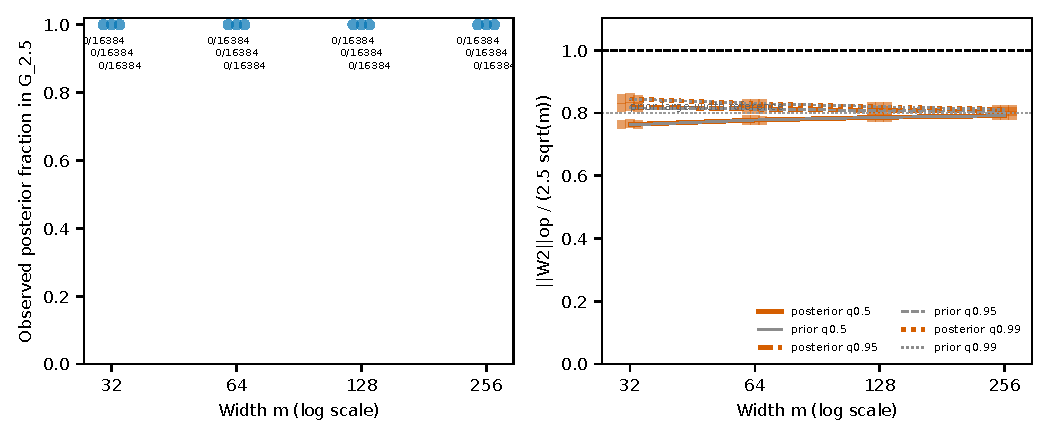
\includegraphics[width=\linewidth]{figures/main_3_spectral.pdf}
\caption{Posterior relevance of the final deep spectral domain. Left: empirical fractions of archived draws from the unrestricted two-hidden-layer posterior satisfying ||W2||op/sqrt(m) <= 2.5, at fixed n=128. 196608 states were inspected, with 0 observed exits in total (per target: m=32 r0: 0, m=32 r1: 0, m=32 r2: 0, m=64 r0: 0, m=64 r1: 0, m=64 r2: 0, m=128 r0: 0, m=128 r1: 0, m=128 r2: 0, m=256 r0: 0, m=256 r1: 0, m=256 r2: 0); counts retain chain identity and are not treated as iid rare-event trials. All inspected states were inside the event; no zero-width interval is reported. Right: the median, 95th, and 99th percentiles of the normalized spectral norm, with matching iid Gaussian-prior reference quantiles. The boundary is one. Posterior/prior comparison: m=32: posterior median 0.763 vs prior 0.762, posterior q99 0.848 (max over replicates); m=64: posterior median 0.777 vs prior 0.778, posterior q99 0.831 (max over replicates); m=128: posterior median 0.786 vs prior 0.786, posterior q99 0.819 (max over replicates); m=256: posterior median 0.791 vs prior 0.791, posterior q99 0.812 (max over replicates). This assesses whether the conditional LSI domain contains a substantial part of the sampled posterior. It does not estimate the theorem's exponential exit-rate constants, and high observed mass does not turn conditional deep LSI into a global statement.}
\label{fig:main_3_spectral}
\end{figure}

% appendix_s1_validation
\begin{figure}[t]
\centering
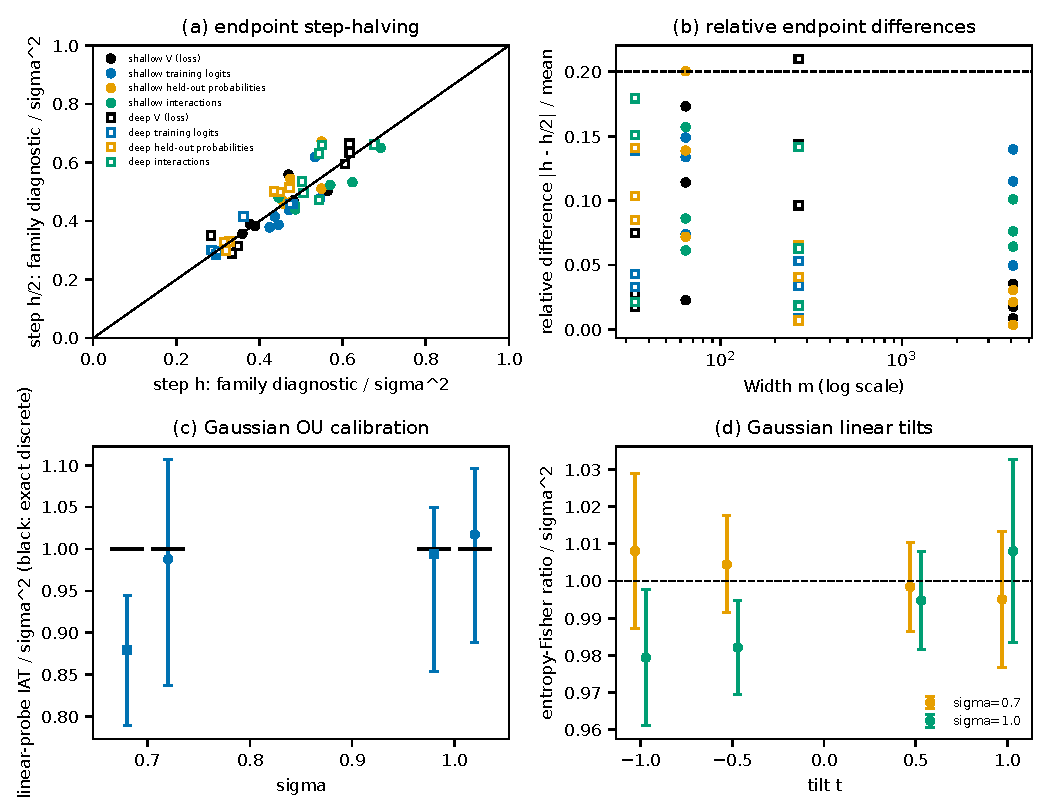
\includegraphics[width=\linewidth]{figures/appendix_s1_validation.pdf}
\caption{Numerical support. (a) Endpoint family relaxation diagnostics at the production step versus half step, normalized by sigma\^{}2, with the identity line (final comparison round shown; 5 family comparisons failed and are listed in tables/endpoint\_comparisons.csv). (b) Relative endpoint differences with the 20\% protocol threshold for all replicates and both architectures. (c) Gaussian OU linear-probe integrated autocorrelation times against the exact discrete value, with bootstrap intervals. (d) Gaussian linear entropy--Fisher ratios at t=-1,-0.5,0.5,1 divided by sigma\^{}2, with the value-one reference.}
\label{fig:appendix_s1_validation}
\end{figure}

% appendix_s2_static_checks
\begin{figure}[t]
\centering
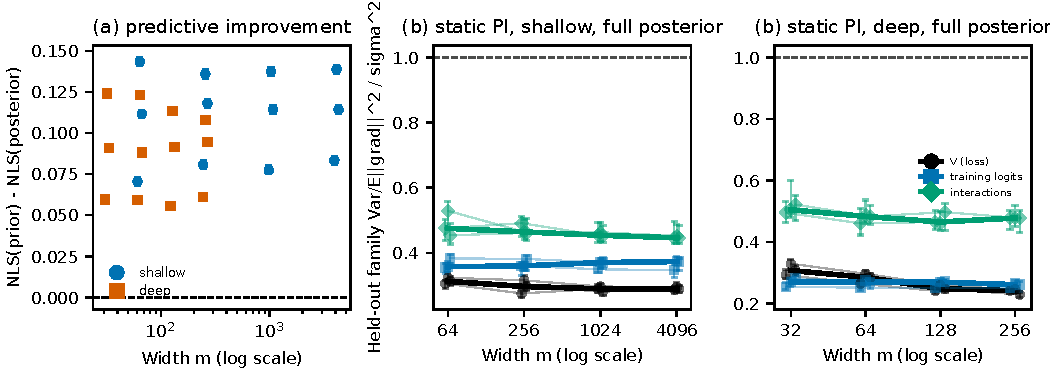
\includegraphics[width=\linewidth]{figures/appendix_s2_static_checks.pdf}
\caption{Appendix checks at no additional sampling cost. (a) Bayesian predictive negative log score of the prior mixture minus that of the posterior on all held-out points (positive: the posterior predicts better); observed range 0.055 to 0.144 nats per point. (b) Held-out family static Poincare ratios Var/E||grad g||\^{}2 on the unrestricted posterior for both architectures, divided by sigma\^{}2; hollow points did not meet the 15\% relative MCSE or reference-validity gate. Small ratios are not upper bounds on the Poincare constant.}
\label{fig:appendix_s2_static_checks}
\end{figure}
